\paragraph{L'interface SocketListener}


\begin{minipage}
    {\linewidth}
    \centering
    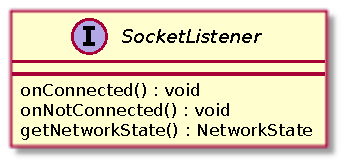
\includegraphics[width=0.30\linewidth]{../schemas/Conception_detaillee/interface_SocketListener.pdf}
    \captionof{figure}{Diagramme de l'interface SocketListener}
\end{minipage}
\subparagraph{Philosophie de conception \newline} 

\medspace

L'interface SocketListener a pour rôle de retourner l'état de la connexion. 

\subparagraph{Description structurelle \newline}

\medspace

\textbf{Attributs :}

N.A.

\textbf{Services offerts :}

\begin{itemize}
    \item \textbf{onConnected() : void} --- Opération qui retourne l'état connecté. 
    \item \textbf{onNotConnected() : void } --- Opération qui retourne l'état non connecté.
    \item \textbf{getNetworkState() : NetworkState } --- Opération qui permet de retourner l'état de la connexion à l'ensemble de l'application. 
\end{itemize}

